%%
%  ******************************************************************************
%  * #file    Szablon_raportu_EN_Latex.tex
%  * #author  Adrian Wójcik   adrian.wojcik(at)put.poznan.pl
%  *          
%  * #commit  Patryk Kościk   koscikpatryk(at)gmail.com
%  *          Modified the template for Projekt przejsciowy purposes          
%  *          
%  * #version 1.0
%  * #date    09-Mar-2022
%  * #brief   PROJPRZEJ
%  *
%  ******************************************************************************
%%  
\documentclass[11pt, a4paper]{article}

\usepackage{setup}

% Wypełnijcie te dyrektywy zgodnie z waszym tematem
% \lab      -> NAZWA CZUJNIKA, np.: 'DHT22'
% \comment  -> Króciutki opis co to, np.: 'Cyfrowy budżetowy czujnik temperatury'
%
\lab{Czujnik ruchu}
\comment{Moduł czujnika ruchu PIR HC-SR501 }
\author{Adam Rewekant}

% Absolutny zakaz dotykania tego tutaj bo jak dotkiecie to coś jebnie
\university{Politechnika Poznańska}
\faculty{Wydział Automatyki, Robotyki i Elektrotechniki}
\institute{Instytut Robotyki i Inteligencji Maszynowej}
\department{Zakład Sterowania i Elektroniki Przemysłowej}
\addbibresource{bib/elem.bib}
\nocite{*}

%%
%
% Początek dokumentu
%
%%
\begin{document}

%% Strona tytułowa %%
\mainpage{{fig/element/mainfot}}

\newpage
\section*{Opis elementu} \addcontentsline{toc}{section}{Wstęp}
Moduł czujnika ruchu PIR HC-SR501 to czujnik promieniowania podczerwonego wykrywający ruch. Zasada działania tego czujnika, polega na generowaniu i wysyłaniu wiązki podczerwieni, która odbija się od przedmiotów, ludzi i zwierząt, które wykazują temperaturę wyższą od temperatury środowiska, w którym przebywają. Jeśli wiązka zostanie odbita w stronę czujnika, wówczas układ sterowania poda na wyjściu stan wysoki. 



\vspace{0.5cm}
\begin{figure}[h]
\centering
\begin{subfigure}{.5\textwidth}
  \centering
  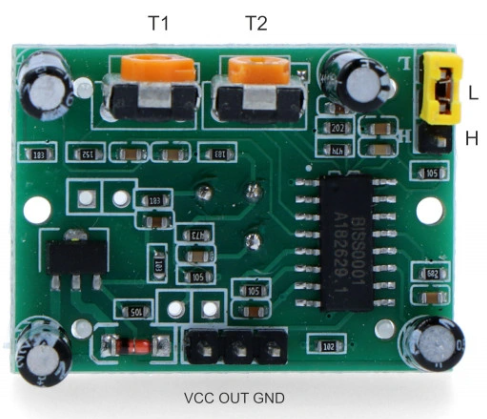
\includegraphics[width=.6\linewidth]{fig/element/fot1.png}
  \caption{HC-SR501 \cite{fot1}}
  \label{fig:sub1}
\end{subfigure}%
\begin{subfigure}{.5\textwidth}
  \centering
  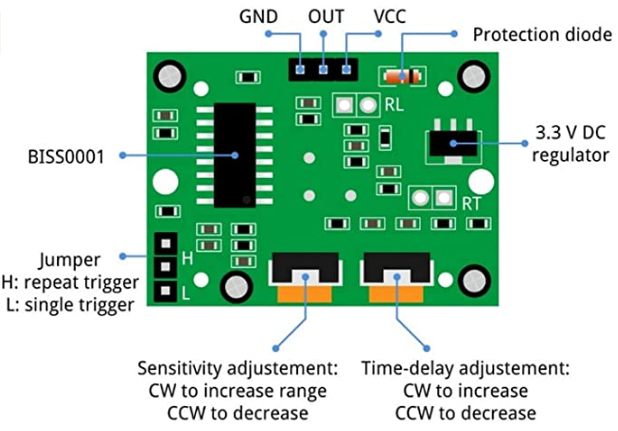
\includegraphics[width=.8\linewidth]{fig/element/fot2.png}
  \caption{HC-SR501 \cite{fot2}}
  \label{fig:sub2}
\end{subfigure}
\caption{Przykładowe zdjęcia czujnika.}
\label{fig:test}
\end{figure}
\vspace{0.5cm}

Istnieje możliwość regulacji parametrów za pomocą potencjometrów:

\begin{itemize}
    \item T1 - czas trwania stanu wysokiego po wykryciu obiektu 
    \item T2 - czułość czujnika (dystans, w którym wykrywa ruch obiektu)
\end{itemize}

Czujnik posiada dwa tryby pracy, które wybierane są za pomocą zwarcia odpowiednich pinów:
\begin{itemize}
    \item retriggering - wyjście osiąga stan wysoki po wykryciu obiektu i jest on utrzymywany przez cały czas wykrywania trwającego ruchu, czujnik domyślnie znajduje się w tym trybie.
    \item non-retriggering  - wyjście osiąga stan wysoki tylko raz po wykryciu obiektu, następnie przechodzi w stan niski niezależnie od tego, czy ruch dalej występuje.
\end{itemize}

\begin{figure}[h]
\centering
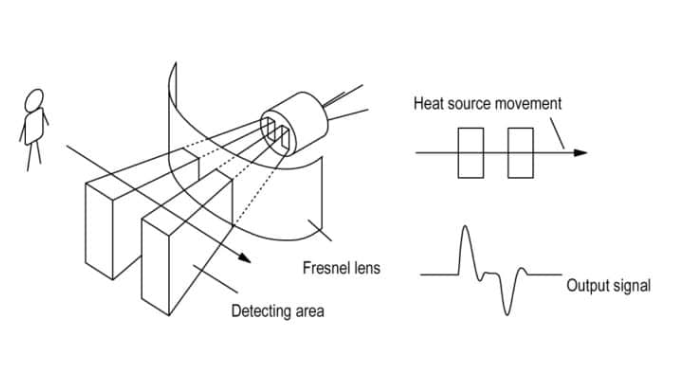
\includegraphics[width=.62\linewidth]{fig/element/dzialanie.png}
\caption{Budowa czujnika.\cite{fot3}}
\label{fig:test}
\end{figure}
\vspace{0.5cm}

\newpage
\section{Użycie czujnika}

\vspace{0.5cm}
\begin{figure}[h!]
    \centering
    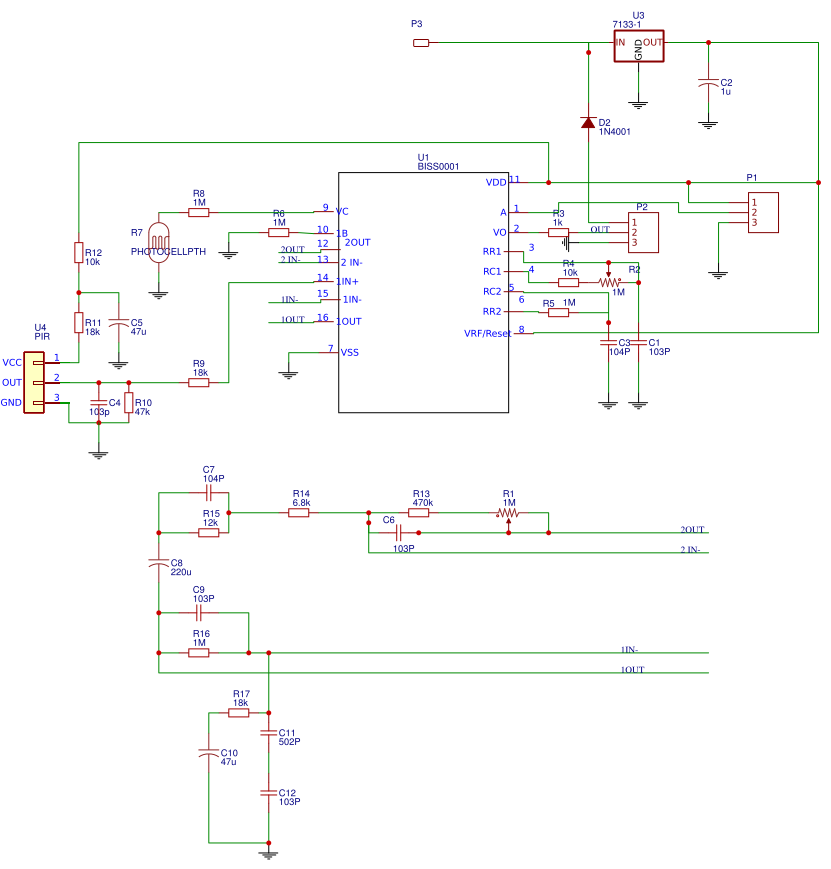
\includegraphics[width=\linewidth]{fig/element/PIRkicad.png}
    \caption{Połaczenie elektryczne}
    \label{fig:my_label}
\end{figure}
\vspace{0.5cm}

Czujnik ruchu, wykorzystywany jest najczęściej do wykrywania obecności człowieka w pomieszczeniach w systemach alarmowych i oświetleniowych.

\newpage
\section{Prezentacja działania układu}

\vspace{0.5cm}
\begin{figure}[h!]
    \centering
    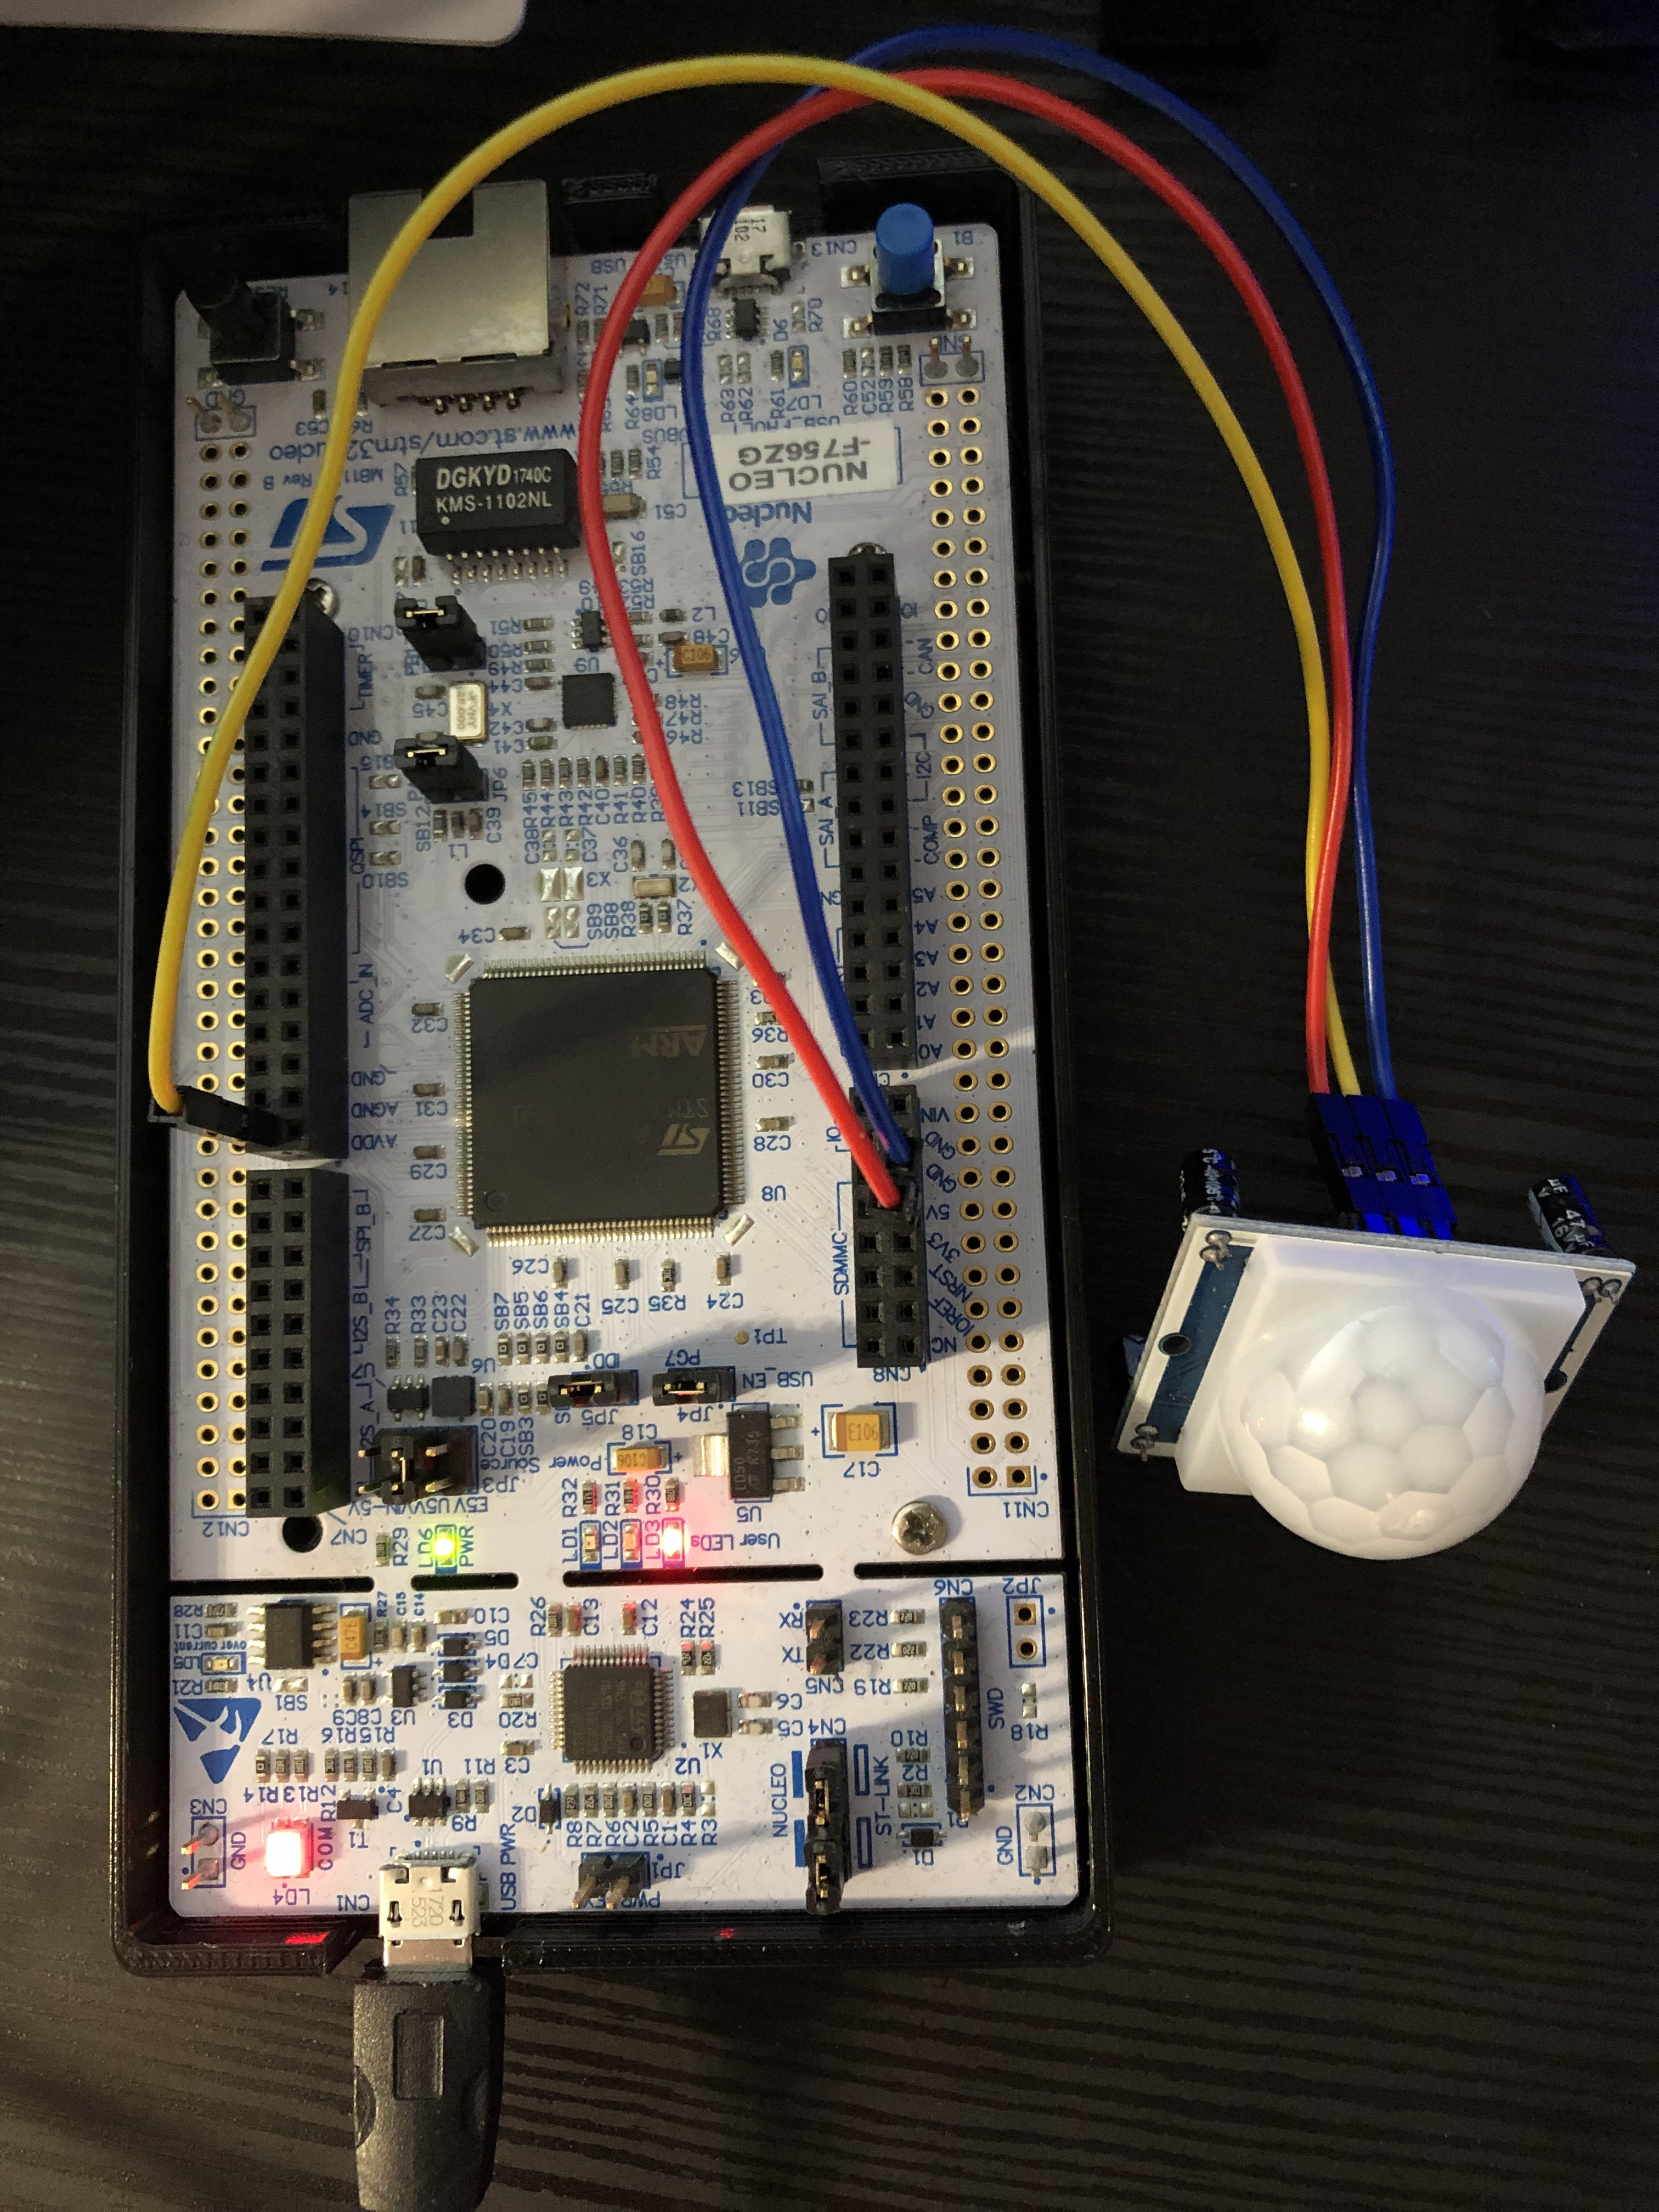
\includegraphics[width=0.8\textwidth]{fig/element/uklad.jpg}
    \caption{Zdjęcie układu.}
    \label{fig:my_label}
\end{figure}

Zakres pomiarowy czujnika to 7 metrów, a jego kąt widzenia wynosi do 100$^\circ$. Jak widać czujnik sygnalizuje wykrycie ruchu co świadczy o poprawnym działaniu układu.\\

Działanie czujnika zostało zaprezentowane na krótkim wideo. \cite{youtube}.
\newpage
\printbibliography[heading=bibintoc]

\end{document}
